\documentclass[12pt]{article}
\usepackage[margin=2.5cm]{geometry}
\usepackage{enumerate}
\usepackage{amsfonts}
\usepackage{amsmath}
\usepackage{fancyhdr}
\usepackage{amsmath}
\usepackage{amssymb}
\usepackage{amsthm}
\usepackage{mdframed}
\usepackage{graphicx}
\usepackage{subcaption}
\usepackage{adjustbox}
\usepackage{listings}
\usepackage{xcolor}
\usepackage{booktabs}
\usepackage[utf]{kotex}
\usepackage{hyperref}

\definecolor{codegreen}{rgb}{0,0.6,0}
\definecolor{codegray}{rgb}{0.5,0.5,0.5}
\definecolor{codepurple}{rgb}{0.58,0,0.82}
\definecolor{backcolour}{rgb}{0.95,0.95,0.92}

\lstdefinestyle{mystyle}{
    backgroundcolor=\color{backcolour},
    commentstyle=\color{codegreen},
    keywordstyle=\color{magenta},
    numberstyle=\tiny\color{codegray},
    stringstyle=\color{codepurple},
    basicstyle=\ttfamily\footnotesize,
    breakatwhitespace=false,
    breaklines=true,
    captionpos=b,
    keepspaces=true,
    numbers=left,
    numbersep=5pt,
    showspaces=false,
    showstringspaces=false,
    showtabs=false,
    tabsize=1
}

\lstset{style=mystyle}

\pagestyle{fancy}
\renewcommand{\headrulewidth}{0.4pt}
\lhead{Hyungmo Gu}
\rhead{CSC369 Week 9 Notes}

\begin{document}
\title{CSC369 Week 9 Notes}
\author{Hyungmo Gu}
\maketitle

\section{Disk I/O}

\begin{itemize}
    \item File system implementation
    \begin{itemize}
        \item Files and directories live on \textbf{secondary storage}
        \begin{itemize}
            \item Anything outisde of ``Primary memory''
            \item Is persistent (or non-volatile): Data survives loss of power
        \end{itemize}
    \end{itemize}
    \item Disk components

    \begin{center}
        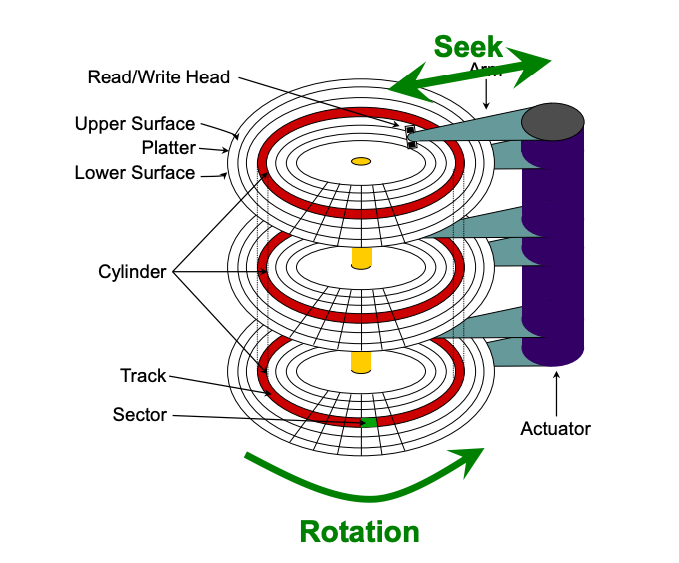
\includegraphics[width=0.8\linewidth]{images/week_9_notes_1_1.png}
    \end{center}

    \begin{itemize}
        \item \textbf{Actuator:} is an electronic device controlled by a motor
        that moves the hard drive head arm. $^{[1]}$
        \item \textbf{Read/Write Heads:} are the small parts of a hard drive which
        move above the disk platter and transform the platter's magnetic field into
        electric current $^{[1]}$

        \begin{center}
            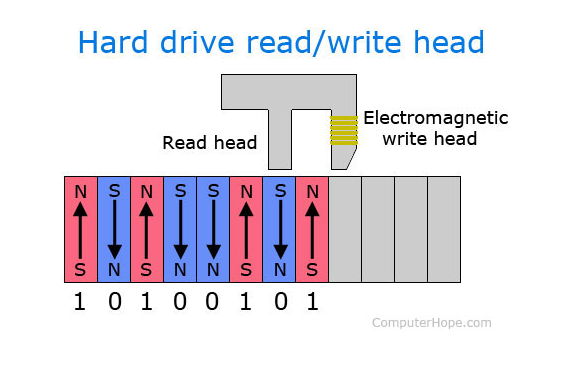
\includegraphics[width=0.8\linewidth]{images/week_9_notes_1_2.png}
        \end{center}

        \item \textbf{Upper Surface:}
        \item \textbf{Lower Surface:}
        \item \textbf{Platter:}
        \item \textbf{Cylinder:}
        \item \textbf{Track:}
        \item \textbf{Sector:}
    \end{itemize}

    \bigskip

    \underline{\textbf{Refernces:}}

    \bigskip

    \begin{enumerate}[1)]
        \item Computer Hope: Actuator, \href{https://www.computerhope.com/jargon/a/actuator.htm}{link}
        \item Andrew. (2018, January 16). \textit{Hard links and Symbolic links — A comparison}. Medium. \href{https://medium.com/@307/hard-links-and-symbolic-links-a-comparison-7f2b56864cdd}{link}
    \end{enumerate}

    % \item Disk service time
    % \item Mixing workloads can be tricky
    % \item Components of disk access time
    % \item Disk are slow
    % \item OS design principles
    % \item Disks are messy
    \item OS $\leftrightarrow$ disk interaction
    \item Logical Block Addressing
    \item Disk Scheduling
    % \item Back to Files and Directories
    % \item Disk Layout Strategies
    % \item Indexed Allocation: Unix Inodes
    % \item Unix Inodes and Path Search
    \item File System Implementation
    \item Original Unix File System
    % \item Data and Inode Placement
    \item FFS
    \item Cylinder Groups
    % \item Space Allocation in Cylinder Groups
    % \item More FFS Solutions
    % \item FFS: Consistency I ssues
    % \item FFS Observation 1
    % \item FFS Observation 2
    \item Log Structured File System (LSF)
    \item NFTS (Windows)
    \item MFT Record
    % \item MFT Record for a Small Directory
    % \item Better I/O performance through parallelism
\end{itemize}

\end{document}